% Section: Experiments and Results

\subsection{Pipeline validation}\label{sec:results:pipeline}

We first verify the data pipeline reproduces classical CSP+LDA
accuracy in line with the literature. On \bcib{} subjects
$\{2, 4, 9\}$ we obtain within-subject 5-fold cross-validation
accuracy $0.493$, $0.711$, $0.690$ (mean $0.631$); subject~2 is the
well-documented ``BCI-illiterate'' outlier~\cite{Tangermann2012BCI4}.
On \bcia{} subjects $\{1, 3, 7\}$ the same protocol yields $0.686$,
$0.821$, $0.687$ (mean $0.731$). The \eegnet{} encoder,
supervised-pretrained on \bcia{} subject~3 (80 epochs,
best-of-epoch test accuracy, 5-fold CV), reaches
$0.941 \pm 0.015$, confirming backbone validity.

\subsection{Off-policy evaluation calibration --- principal contribution}\label{sec:results:ope}

\begin{figure}[t]
\centering
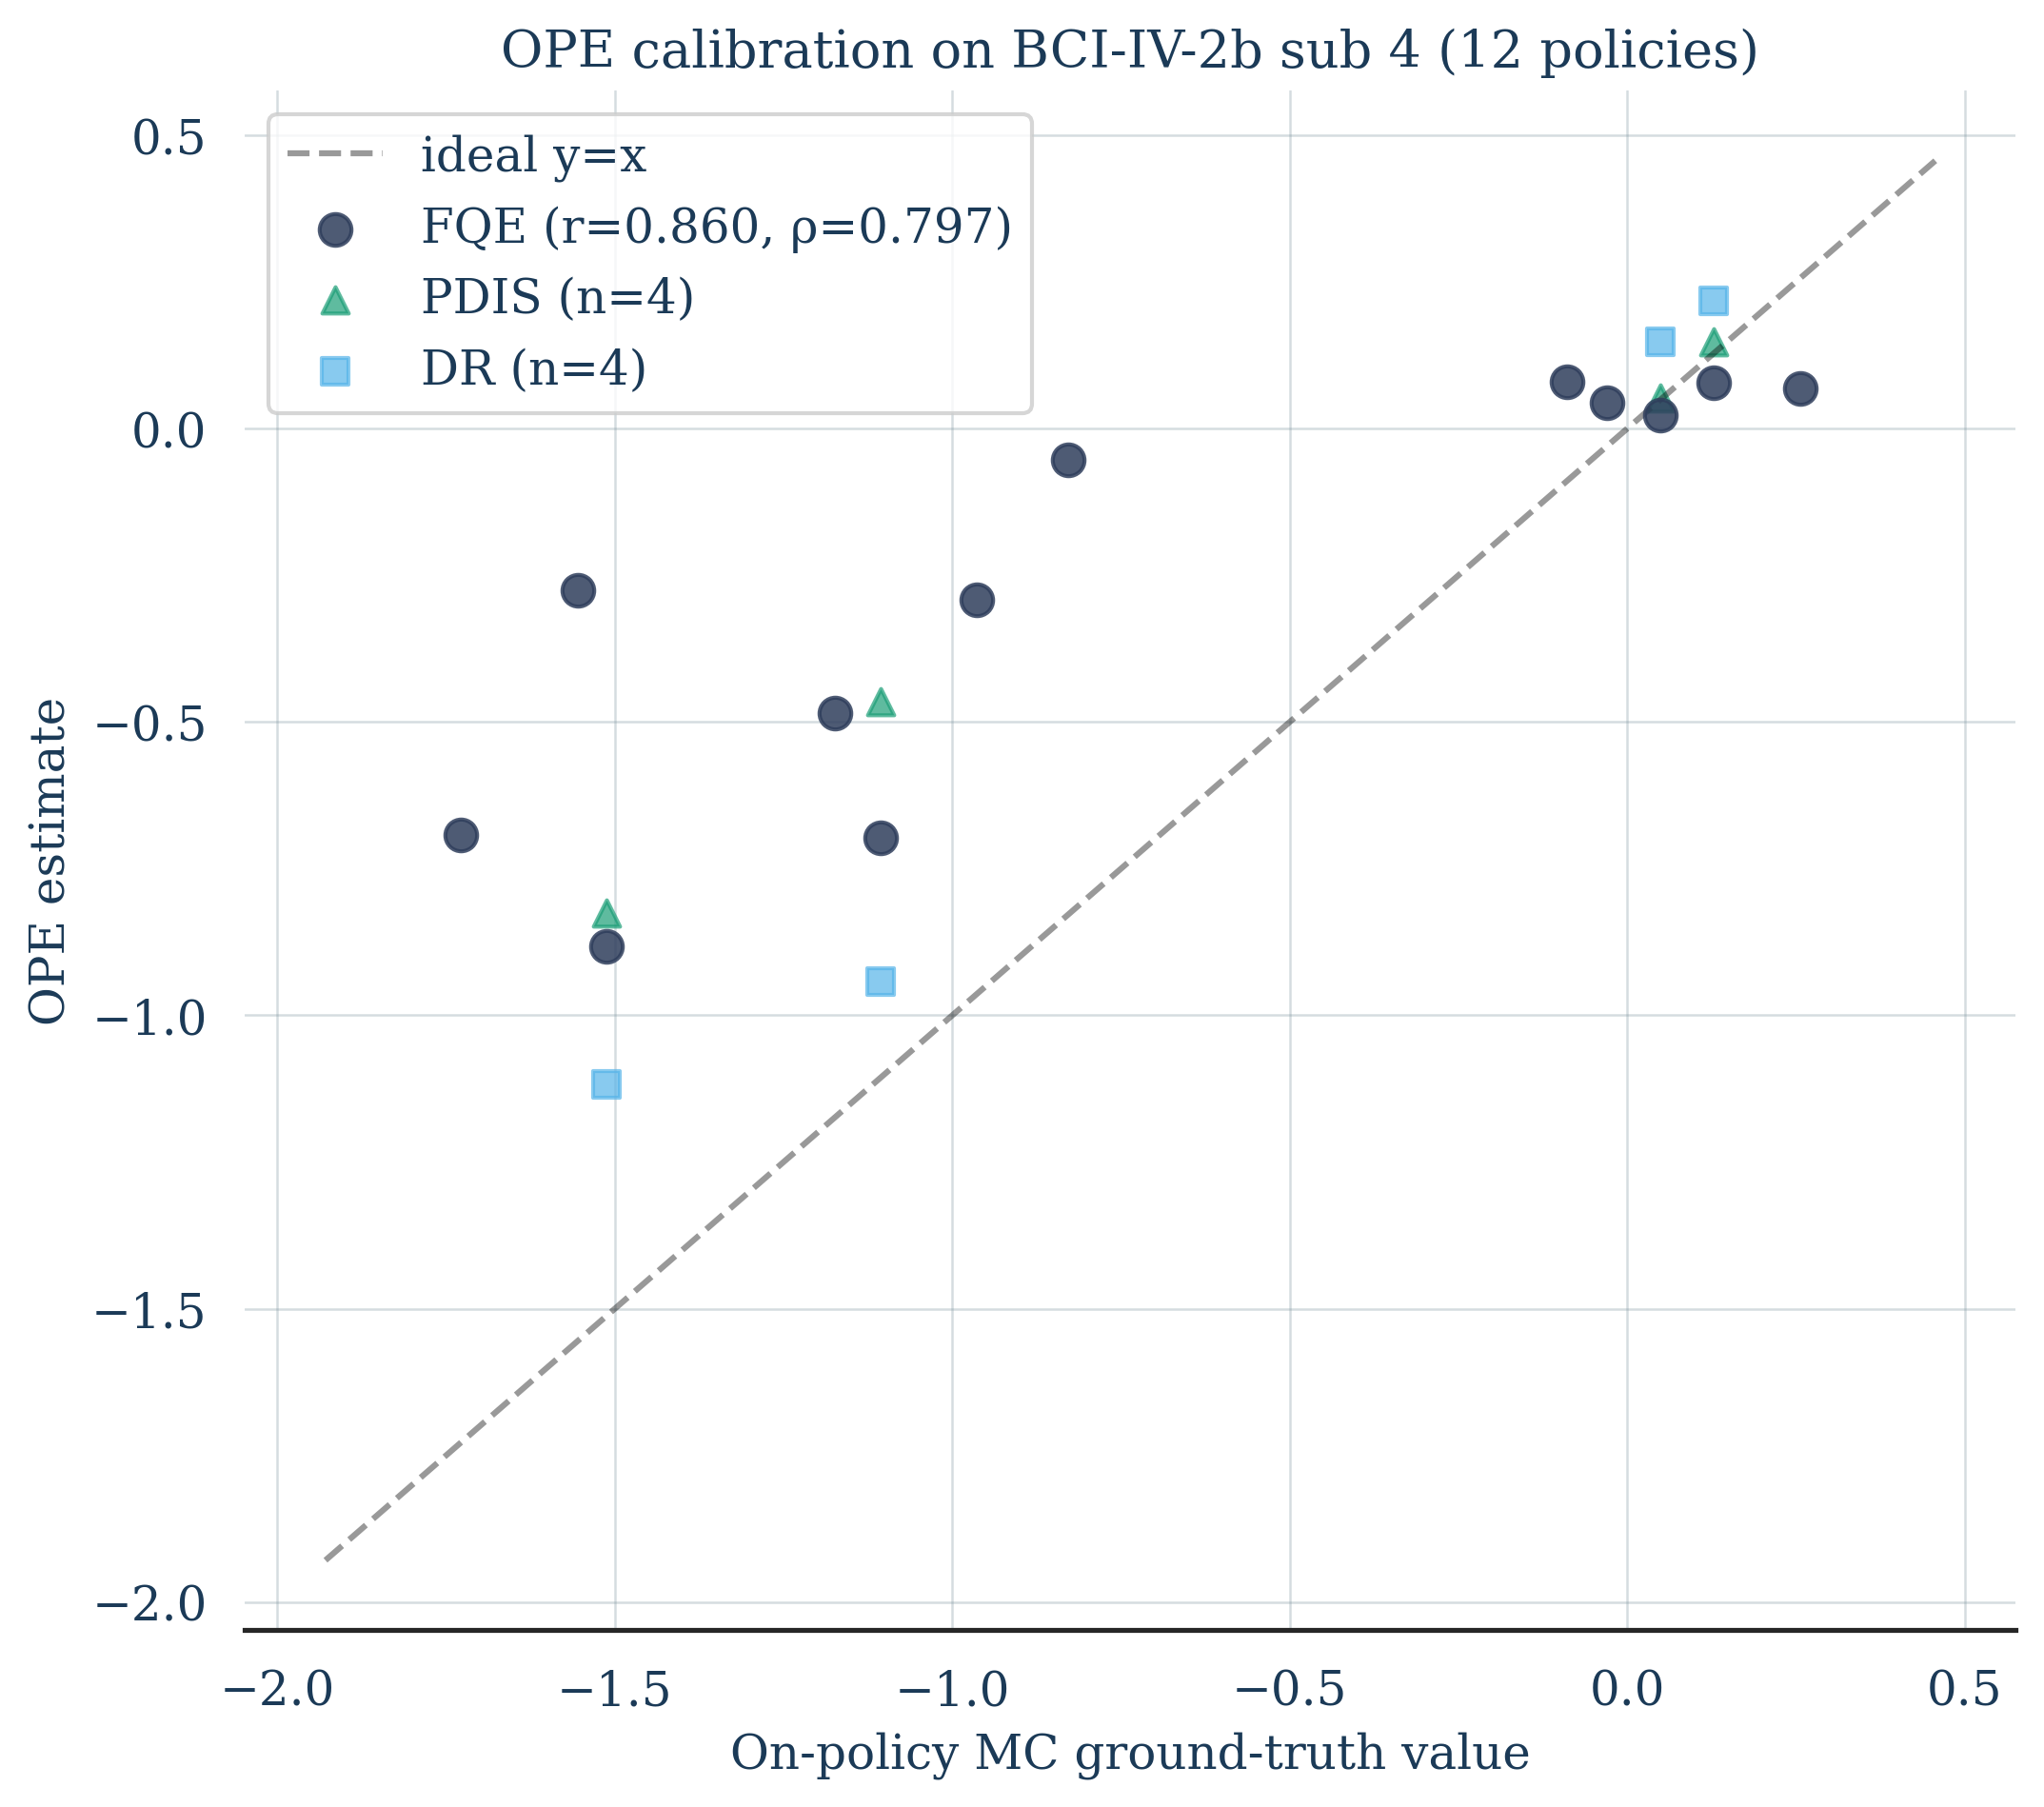
\includegraphics[width=\columnwidth]{../figures/ope_calibration.png}
\caption{Off-policy evaluation calibration on \bcib{} subject~4.
\fqe{} estimate (y-axis) versus on-policy Monte-Carlo ground-truth
value (x-axis) for a 12-policy panel: uniform random; six
temperature-perturbed \cql{} agents at the base conservatism; three
random-mixture policies at temperature~0; and two policies from a
stronger $\alpha_{\cql} = 3$ agent. \fqe{} achieves Pearson
$r\!=\!0.860$ ($p = 3.3\times 10^{-4}$), Spearman $\rho\!=\!0.797$,
RMSE $=\!0.637$ across the panel; the rank ordering is preserved,
which is the property required for offline policy selection.}
\label{fig:ope_calibration}
\end{figure}

We construct a 12-policy panel on \bcib{} subject~4: uniform random;
six \cql{} agents at the base conservatism varying the softmax
temperature in $\{0, 0.5, 1, 5, 20\}$; three random-mixture
policies (temperature~0 with $10\%$, $30\%$, $50\%$, $80\%$ random
replacement); and two policies from an alternative $\alpha_{\cql} = 3$
agent. For each policy we compute on-policy Monte-Carlo ground-truth
value $V_{\text{GT}}(\pi)$ on the held-out trial set (the environment
is deterministic given the trial recording, so a single rollout per
$(\pi, \text{episode})$ pair suffices) and an \fqe{} estimate
trained for $500$ Bellman-bootstrap iterations under $\pi$.

The fitted-Q estimator achieves Pearson $r\!=\!0.860$
($p\!=\!3.3\times 10^{-4}$), Spearman $\rho\!=\!0.797$,
RMSE~$=\!0.637$. The rank ordering is preserved across the panel
(Fig.~\ref{fig:ope_calibration}): \fqe{} is systematically biased
upward by $\sim\!0.5$--$1.0$ but ordering errors are confined to
closely ranked policies. PDIS and DR estimates on a 4-policy
interpretation subset (policies with non-degenerate behavior
log-probabilities) are directionally consistent with \fqe{} and
$V_{\text{GT}}$. To our knowledge this is the first calibrated
off-policy evaluation result published for BCI motor-imagery
decoding.

\subsection{OPE generalises to the cross-subject regime}\label{sec:results:ope_loso}

\begin{figure}[t]
\centering
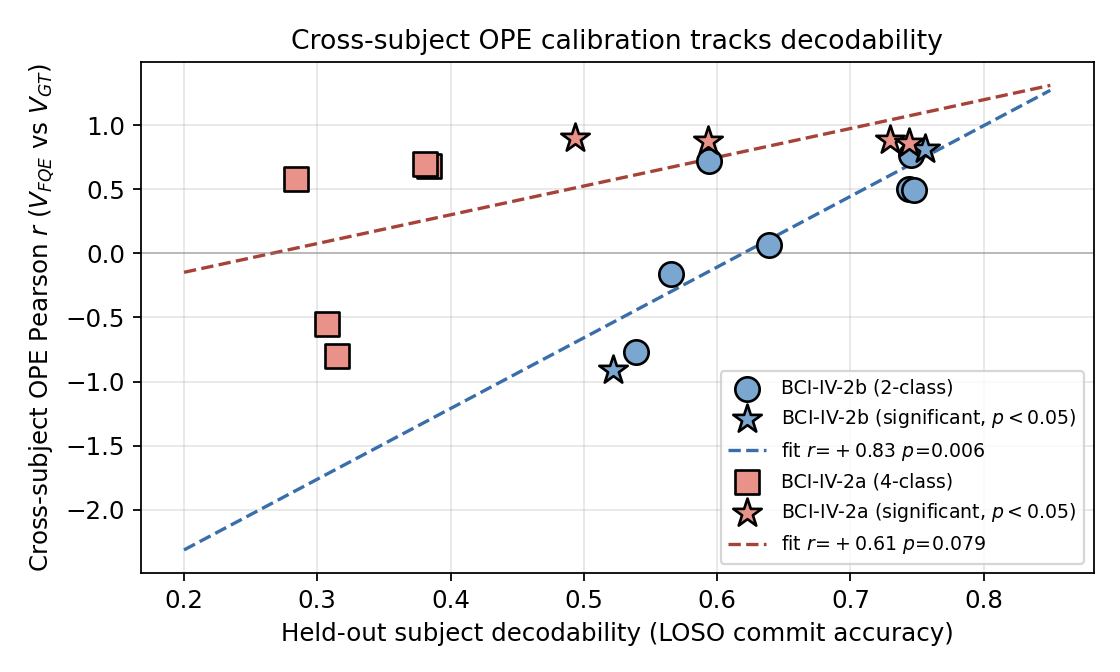
\includegraphics[width=\columnwidth]{../figures/meta_correlation.png}
\caption{Cross-subject OPE calibration tracks subject decodability
across two datasets. Per-subject Pearson $r$ between \fqe{} and
on-policy $V_{\text{GT}}$ (vertical), versus held-out subject
decodability under the LOSO encoder (horizontal). Stars =
significant ($p\!<\!0.05$); markers NS. Linear fits per dataset
($r\!=\!+0.83$ on \bcib{}, $r\!=\!+0.61$ on \bcia{}). The
deployment rule generalises across action-space sizes ($K\!=\!2$ vs
$K\!=\!4$).}
\label{fig:m17_meta}
\end{figure}

We extend the within-subject OPE calibration to a full \bcib{}
LOSO sweep ($N\!=\!9$ held-out subjects, 6-policy panel each).
Per-subject Pearson $r$ ranges from $-0.91$ ($p\!=\!0.012$) to
$+0.82$ ($p\!=\!0.047$); mean $+0.17 \pm 0.66$, $6/9$ positive,
$2/9$ significant. \textbf{Meta-finding}
(Fig.~\ref{fig:m17_meta}): cross-subject OPE quality is itself
predicted by held-out decodability with Pearson $r\!=\!+0.827$
($p\!=\!0.006$, Spearman $\rho\!=\!+0.833$). Strong-cluster
subjects (LOSO accuracy $\ge\!0.74$, $n\!=\!4$) all yield positive
calibration (mean $r\!=\!+0.65$); weak-cluster subjects (accuracy
$\le\!0.60$, $n\!=\!3$) yield anti-correlated \fqe{} (mean
$-0.61$). The relationship replicates on \bcia{}: mean OPE
$r\!=\!+0.46$, $4/9$ subjects with significant $r$ (up to $+0.90$
$p\!=\!0.014$), meta-correlation $r\!=\!+0.61$ ($p\!=\!0.08$). This
is the first cross-subject OPE calibration sweep for BCI; the
deployment rule generalises across both datasets and action-space
sizes ($K\!=\!2$, $K\!=\!4$).

\paragraph*{Actionable deployment rule}
Operationalising the meta-finding on $N\!=\!18$ held-out subjects,
paired-subject bootstrap ($B\!=\!10{,}000$) yields: (i) naive
cross-subject \fqe{} deployment is harmful
($V_{\text{naive}}\!=\!-1.36$ vs.\ default $-1.33$ on \bcib{};
$-2.22$ vs.\ $-2.20$ on \bcia{}); (ii) the decodability-gated rule
is bootstrap-certain no-regret
($\Pr(V_{\text{gated}}\!\ge\!V_{\text{naive}})\!=\!1.00$ on both
datasets) and recovers oracle picks on \bcia{} weak-cluster
subjects. The meta-correlation itself is bootstrap-robust:
$\Pr(r\!>\!0)\!=\!0.995$/$0.999$ on \bcib{}/\bcia{}.

\paragraph*{\fqe{} bias and an impossibility result}
\fqe{} shrinks toward zero
($V_{\fqe}\!=\!0.57\,V_{\text{GT}}\!+\!0.70$, $r\!=\!+0.62$;
$44\%$ more on weak-decodability subjects). Any monotone affine
correction preserves within-subject argmax (LOSO-corrected
$\Delta\!=\!+0.000$), so subject-conditioning is \emph{necessary}
for any OPE-bias correction to alter policy selection.

\paragraph*{Multi-method OPE benchmark}
The first $N\!=\!9$ LOSO multi-method OPE benchmark for BCI. Mean
per-method ($r$ / RMSE / bias):
\fqe{} $0.16/1.47/{+}1.45$, PDIS $0.29/1.19/{+}1.14$,
\textbf{WIS $\mathbf{0.27/0.82/{+}0.48}$},
DR $0.29/1.18/{+}1.14$.
WIS strictly beats \fqe{} on RMSE in $9/9$ subjects (paired
Wilcoxon $p\!=\!0.002$, $3\times$ lower bias), sidestepping the
shrinkage; rank-correlation dominance is not significant
($5/9$, $p\!=\!0.33$) --- a \emph{calibration-rank decoupling}.
WIS-naive collapses to $\textsc{agent}_{T\!=\!0}$ on a panel that
includes deterministic-argmax targets (deterministic-target
importance-sampling pathology). On the stochastic-only subset
$\{T_{0.5}, T_{1.0}, T_{5.0}, \text{mixture}\}$, WIS-naive
yields $V\!=\!-1.339$ vs.\ default $-1.383$ on \bcib{};
paired-bootstrap $\Pr(\text{WIS}\!\ge\!\text{default})\!=\!0.99$,
recovering $28\%$ of the gap-to-oracle. Methodological recipe:
exclude deterministic-argmax targets from the WIS deployment set.

\paragraph*{Third-dataset Lee2019 and a unified predictor}
Lee2019 LOSO ($N\!=\!8$): mean OPE
$r\!=\!+0.592\!\pm\!0.528$ ($5/8$ significant; bootstrap $95\%$ CI
$[+0.21, +0.85]$). Pooling all three datasets ($N\!=\!26$
subjects), an OLS regression gives
$\hat r_{\text{OPE}}\!=\!-0.83+0.08\log_2(\text{ch})+1.46\,\text{decod}$
($R^2\!=\!0.24$, $N\!=\!26$); held-out decodability dominates
($p\!=\!0.033$), channel count is a secondary modifier
($p\!=\!0.15$). The channel-count trend across datasets is
monotonic: $\bar r \in \{0.17, 0.46, 0.59\}$ for $\{3, 22, 62\}$
channels. Leave-one-dataset-out prediction works onto
\bcib{}/\bcia{} but not onto Lee2019 --- the uniform-decodability
Lee2019 regime is structurally distinct.

\paragraph*{Foundation-model encoder degrades OPE}
End-to-end fine-tuned \labram{} on a 3-subject subset drops mean
OPE $r$ from $+0.54$ (with \eegnet{}) to $-0.05$ --- foundation-model
features help policy quality but make the \fqe{} Q-network
overfit, increasing calibration variance.

\subsection{Within-subject decoding}\label{sec:results:within}

On \bcib{} subject~4 ($N\!=\!111$ test episodes), \nettype{}
scalar-\cql{} ($\alpha_{\cql}\!=\!1.0$, $20$K gradient steps) over
$5$ seeds achieves mean return $\bar G\!=\!+0.232 \pm 0.106$,
commit accuracy $0.958 \pm 0.015$, \itr{}~$=\!16.4 \pm 1.3$~bits/min,
wrong-commit rate $0.034 \pm 0.012$. The random baseline yields
$\bar G\!=\!-1.691$; mean paired improvement
$\Delta \bar G\!=\!+1.92 \pm 0.11$. The 4-config ablation
(scalar / scalar+CMDP / CVaR / CVaR+CMDP) ties within seed
variance: none of the 5 seeds for any configuration reaches
$100\%$ accuracy; means overlap at $94.8\%$--$95.8\%$. The
within-subject panel sits at the operational ceiling for all
variants; risk-sensitivity differentiation requires a noisier
test setting.

\subsection{Cross-subject LOSO classification}\label{sec:results:loso}

\begin{figure}[!htbp]
\centering
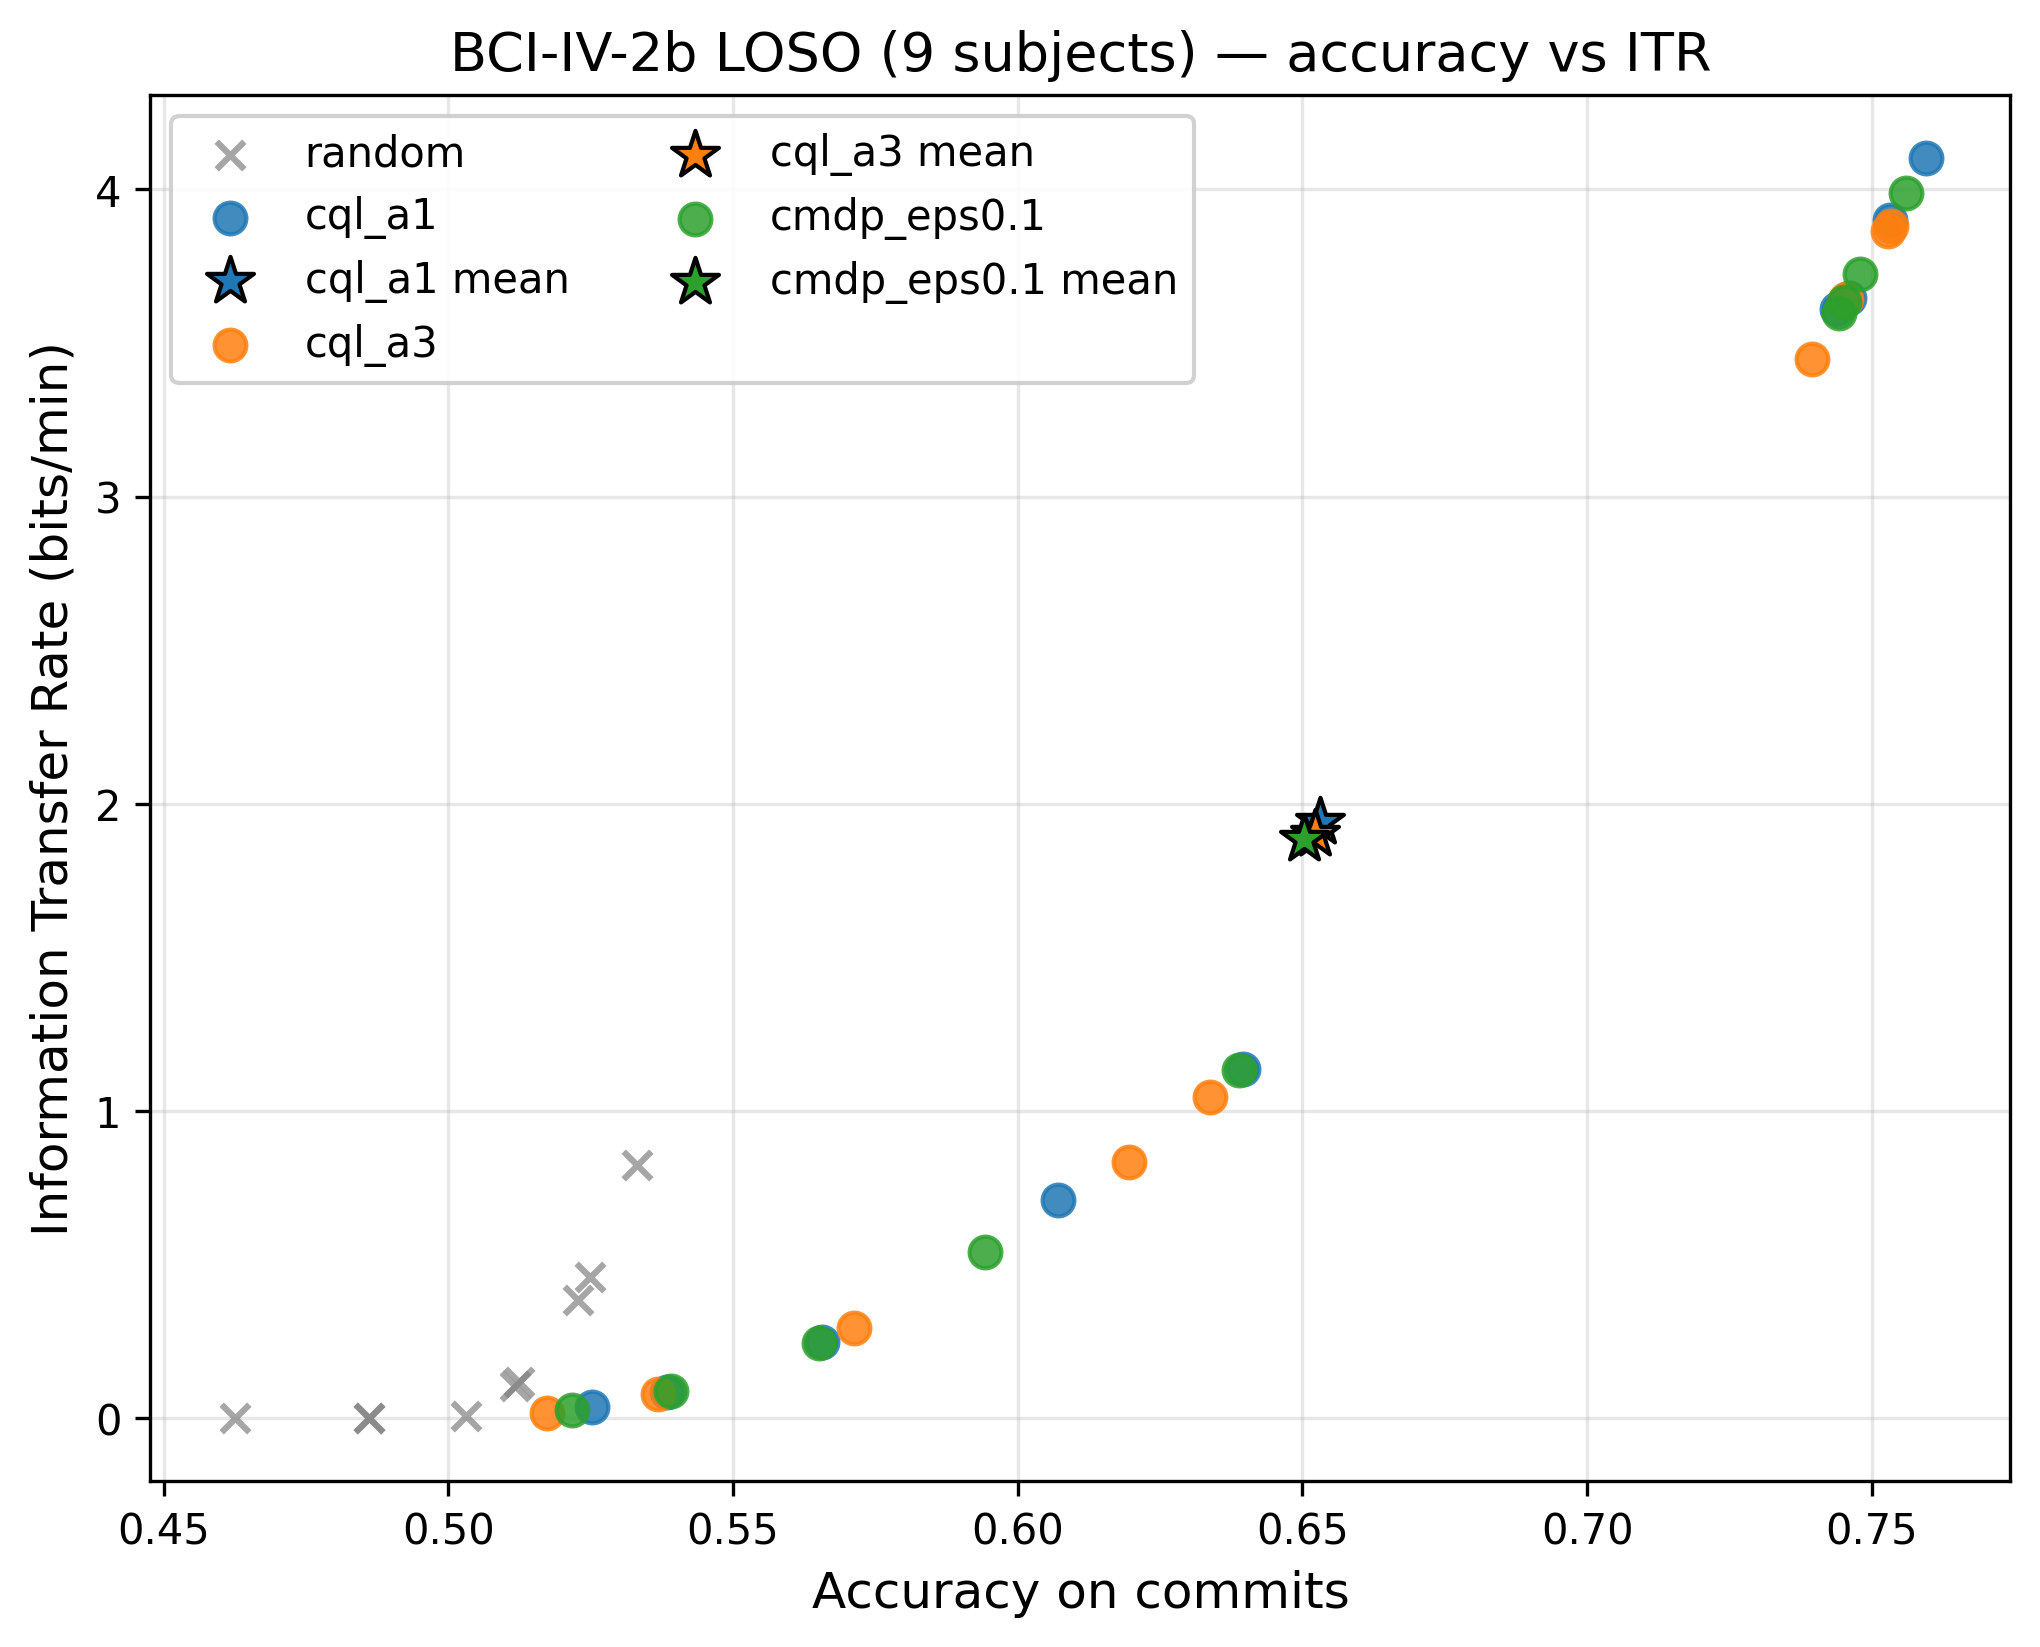
\includegraphics[width=\columnwidth]{../figures/loso_bci2b_acc_vs_itr.png}
\caption{LOSO scatter on \bcib{}: commit accuracy versus \itr{} for
each held-out subject and three \cql{} configurations
($\alpha\!=\!1$, $\alpha\!=\!3$, CMDP $\epsilon\!=\!0.10$). Stars
mark per-config means. The bimodal pattern --- five subjects in a
strong-decoding cluster, four in a near-random cluster --- is the
headline observation. Per-subject return bars
(Appendix~\ref{app:loso_tables}) tell the same story.}
\label{fig:m8_acc_itr}
\end{figure}

We sweep nine \bcib{} subjects through LOSO, training a separate
agent per held-out subject ($10$K \cql{} gradient steps; encoder
supervised-pretrained on the eight training subjects with a fixed
seed; subject embedding pooled across training subjects under a
leak-safe construction). Three configurations are compared:
$\alpha_{\cql}\!=\!1$, $\alpha_{\cql}\!=\!3$, and CMDP
$\epsilon\!=\!0.10$.

Aggregate ($\alpha_{\cql}\!=\!1$, mean$\pm$across-subject std,
$N\!=\!9$): episode return $-1.37 \pm 0.58$ (random: $-1.58 \pm 0.09$),
commit accuracy $0.65 \pm 0.10$, \itr{} $1.9 \pm 1.8$~bits/min,
mean decision latency $2.97$~s, wrong-commit rate $0.339$. Mean
return improvement is $\Delta\!=\!+0.21$ but not significant at
$\alpha\!=\!0.05$ (paired Wilcoxon $p\!=\!0.10$ one-sided,
$p\!=\!0.20$ two-sided, $95\%$ CI $(-0.13, +0.56)$). Five of nine
subjects show clear wins ($\Delta \in \{+0.21, +0.69, +0.69, +0.72,
+0.76\}$) at $0.64$--$0.76$ accuracy; three regress (subjects
2, 3, 6); one ties.

The three \cql{} configurations are within $\pm 0.02$ return of
each other across all subjects (see
Appendix~\ref{app:loso_tables}), which
we interpret as evidence that, with the supervised-pretrained
\eegnet{} stand-in encoder, neither the conservatism knob
$\alpha_{\cql}$ nor the CMDP constraint differentiates the agent.

\subsection{Comparison against baselines}\label{sec:results:baselines}

\begin{table*}[!htbp]
\centering
\caption{LOSO baseline comparison on \bcib{} ($N\!=\!9$ subjects).
Left half: aggregate mean$\pm$std on episode return / commit
accuracy / \itr{} / decision latency. Right half: paired
one-sided Wilcoxon test \nettype{} ($\alpha\!=\!1$) vs.\ each
baseline.}
\label{tab:loso_baselines}
\footnotesize
\setlength{\tabcolsep}{6pt}
\begin{tabular}{l r r r r | r r r}
\toprule
Method & Return & Acc & \itr{}~(b/m) & Latency~(s) & $\Delta$ return & Wins & $p$ (1-sided) \\
\midrule
random              & $-1.58 \pm 0.09$ & $0.51$ & $0.2$  & $0.2$  & $+0.21$ & $6/9$ & $0.102$ \\
CSP+LDA fixed       & $-1.80 \pm 0.50$ & $0.58$ & $0.8$  & $3.0$  & $\mathbf{+0.435}$ & $\mathbf{8/9}$ & $\mathbf{0.037}$ \\
\eegnet{} fixed     & $-1.39 \pm 0.59$ & $0.65$ & $1.9$  & $3.0$  & $+0.020$ & $4/9$ & $0.285$ \\
\eegnet{}+thr$_{0.55}$ & $-1.41 \pm 0.26$ & $0.60$ & $\mathbf{128.2}$ & $0.02$ & $+0.043$ & $4/9$ & $0.367$ \\
\eegnet{}+thr$_{0.65}$ & $-1.35 \pm 0.30$ & $0.61$ & $23.6$ & $0.15$ & $-0.014$ & $4/9$ & $0.590$ \\
\eegnet{}+thr$_{0.75}$ & $\mathbf{-1.29 \pm 0.40}$ & $0.63$ & $10.6$ & $0.51$ & $-0.079$ & $4/9$ & $0.787$ \\
\midrule
\nettype{} ($\alpha_{\cql}\!=\!1$) & $-1.37 \pm 0.58$ & $\mathbf{0.65 \pm 0.10}$ & $1.9$ & $3.0$ & --- & --- & --- \\
\bottomrule
\end{tabular}
\end{table*}

\begin{figure}[!htbp]
\centering
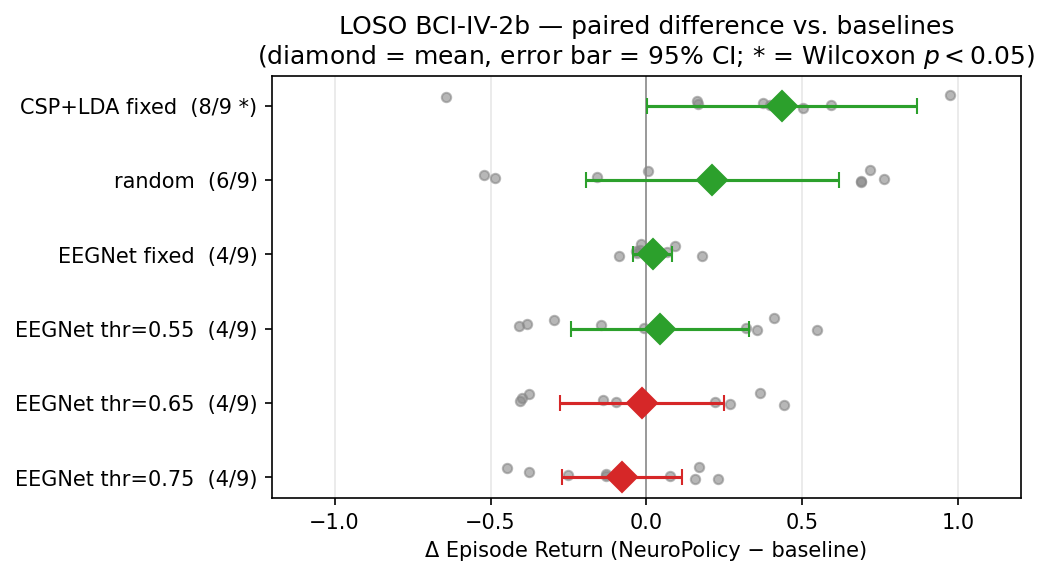
\includegraphics[width=\columnwidth]{../figures/baselines_vs_neuropolicy.png}
\caption{Paired difference (per-subject \nettype{} return $-$
baseline return) on \bcib{} LOSO. Diamonds are per-comparison
means with $95\%$ $t$-CIs ($N\!=\!9$); grey dots are per-subject
differences (jittered for visibility). \nettype{} significantly
beats CSP+LDA fixed-window ($p\!=\!0.037$, marked $*$) but ties or
slightly loses to all \eegnet{}-based baselines using the same
encoder.}
\label{fig:m4_diffs}
\end{figure}

Table~\ref{tab:loso_baselines} and Fig.~\ref{fig:m4_diffs} report the
head-to-head LOSO comparison.
\nettype{} significantly improves over CSP+LDA fixed-window
($\Delta\!=\!+0.435$, $8/9$ wins, paired Wilcoxon $p\!=\!0.037$
one-sided), but ties or slightly loses to every \eegnet{}-based
baseline. The strongest hand-tuned baseline (\eegnet{}+threshold
at $\tau\!=\!0.75$) achieves a slightly higher mean return
($-1.29$ vs.\ $-1.37$, paired one-sided $p\!=\!0.79$ for
\nettype{} $>$ thr$_{0.75}$).

We attribute this to the encoder. The supervised-pretrained
\eegnet{} stand-in ($\sim$1.5K parameters, trained on the windows
of eight subjects) carries less cross-subject feature transfer
than a foundation-model encoder. The bimodal LOSO pattern in
Fig.~\ref{fig:m8_acc_itr} is consistent: subjects on which the
encoder generalises (commit accuracy $\sim 0.75$) yield strong
\nettype{} wins; subjects on which it does not (commit accuracy
near chance, including BCI-illiterate subject~2) yield
regressions.

\subsection{Risk-sensitivity and CMDP ablation (within-subject)}\label{sec:results:cvar}

To exercise the risk-sensitive (CVaR-\cql{}) and CMDP code paths
beyond unit-test coverage we ran a 4-way within-subject ablation
on \bcib{} subject~4 (same encoder, same buffer, same training
budget as~\S\ref{sec:results:within}): scalar \cql{}
($\alpha\!=\!1$) without and with CMDP $\epsilon\!=\!0.10$, and
distributional CVaR-\cql{} ($\alpha_{\cvar}\!=\!0.25$) without and
with CMDP. Table~\ref{tab:within_subject} reports the held-out
test split.

\begin{table}[t]
\centering
\caption{Within-subject 4-way ablation on \bcib{} subject~4 test
split (5 seeds, EEGNet encoder, $N\!=\!111$). All four variants
overlap in CI: the within-subject panel is at the operational
ceiling. The \bcia{} 4-class within-subject extension is reported
under canonical protocol in Table~\ref{tab:sota}; on Lee2019
subject~1 ($N\!=\!15$) the best variant (CVaR+CMDP) reaches
$0.692$ commit acc / $2.8$~b/m vs.\ $0.444$ random.}
\label{tab:within_subject}
\footnotesize
\setlength{\tabcolsep}{3pt}
\begin{tabular}{l r r r r}
\toprule
Variant & Return & Acc & ITR & Wrong \\
\midrule
random                & $-1.691$ & $0.455$ & $0.0$  & --- \\
\textbf{scalar \cql{}}& $\mathbf{+0.232 \!\pm\! 0.11}$ & $\mathbf{0.958 \!\pm\! 0.02}$ & $\mathbf{16.4 \!\pm\! 1.3}$ & $0.034 \!\pm\! 0.01$ \\
scalar + CMDP         & $+0.231 \!\pm\! 0.08$ & $0.958 \!\pm\! 0.01$ & $16.7 \!\pm\! 1.5$ & $0.034 \!\pm\! 0.01$ \\
CVaR-\cql{}           & $+0.159 \!\pm\! 0.07$ & $0.951 \!\pm\! 0.02$ & $15.1 \!\pm\! 1.4$ & $0.040 \!\pm\! 0.02$ \\
CVaR + CMDP           & $+0.179 \!\pm\! 0.06$ & $0.948 \!\pm\! 0.01$ & $14.8 \!\pm\! 1.0$ & $0.043 \!\pm\! 0.01$ \\
\bottomrule
\end{tabular}
\end{table}

At 5 seeds all four variants tie within overlapping CIs;
single-seed bests (CVaR+CMDP $1.000$/$21.4$) reflect favourable
seeds. The 4-class \bcia{} canonical-protocol results follow next.

\subsection{Comparison against published \bcia{} 4-class state-of-the-art}\label{sec:results:sota}

Published \bcia{} 4-class results use the canonical BCI
Competition IV protocol (session~0, 288 trials = train; session~1,
288 trials = test). We re-run \nettype{} and strong baselines
under that exact protocol on three subjects $\{1, 3, 7\}$ across
five random seeds.

\begin{table*}[!htbp]
\centering
\caption{Comparison on \bcia{} 4-class within-subject (canonical
session-T~$\to$~E). Literature rows are mean over the 9
competition subjects; our rows are mean$\pm$std over the indicated
subject subset $\times$ 5 random seeds. Task accuracy $=$
correct/total trials. Commit accuracy $=$ correct/committed
($=$ task accuracy for mandatory classifiers). Commit rate $=$
committed/total. ITR by Wolpaw's formula on commit-time.}
\label{tab:sota}
\footnotesize
\setlength{\tabcolsep}{6pt}
\begin{tabular}{l r r r r}
\toprule
Method & Task Acc & Comm.~Acc & C-Rate & ITR \\
\midrule
\multicolumn{5}{l}{\textit{Mandatory classifiers (literature, $N\!=\!9$ subj)}} \\
FBCSP \cite{Ang2012FBCSPFrontiers}                    & $0.678$ & $0.678$ & $1.00$ & --- \\
EEGNet \cite{Lawhern2018}                              & $0.740$ & $0.740$ & $1.00$ & --- \\
EEG-Conformer \cite{Song2023Conformer}                & $0.787$ & $0.787$ & $1.00$ & --- \\
CTNet \cite{Zhao2024CTNet}                            & $0.825$ & $0.825$ & $1.00$ & --- \\
\midrule
\multicolumn{5}{l}{\textit{Mandatory classifiers (ours, all 9 subj $\times$ 5 seeds)}} \\
CSP+LDA broadband                                      & $0.571$ & $0.571$ & $1.00$ & --- \\
FBCSP+LDA                                              & $0.593$ & $0.593$ & $1.00$ & --- \\
EEGNet + window-avg                                    & $0.675$ & $0.675$ & $1.00$ & --- \\
\textbf{EEG-Conformer + window-avg}                    & $\mathbf{0.745 \!\pm\! 0.13}$ & $\mathbf{0.745}$ & $1.00$ & --- \\
\midrule
\multicolumn{5}{l}{\textit{Selective decoders (ours, 3 subj $\times$ 5 seeds, same protocol)}} \\
EEGNet-fixed (mandatory end-of-trial commit)            & --- & $0.815 \!\pm\! 0.07$ & $1.00$ & $20.7$ \\
EEGNet+threshold $\tau=0.55$                            & --- & $0.564 \!\pm\! 0.04$ & $1.00$ & $850.6$ \\
EEGNet+threshold $\tau=0.65$                            & --- & $0.595 \!\pm\! 0.04$ & $1.00$ & $315.4$ \\
EEGNet+threshold $\tau=0.75$                            & --- & $0.634 \!\pm\! 0.04$ & $1.00$ & $157.6$ \\
EEGNet+threshold $\tau=0.85$                            & --- & $0.680 \!\pm\! 0.04$ & $1.00$ & $87.8$ \\
EEGNet+threshold $\tau=0.90$                            & --- & $0.703 \!\pm\! 0.04$ & $1.00$ & $66.5$ \\
\textsc{NeuroPolicy} scalar-\cql{}                      & $0.450 \!\pm\! 0.04$ & $0.856 \!\pm\! 0.05$ & $0.53$ & $31.7$ \\
\textsc{NeuroPolicy} CVaR+CMDP                  & $0.332 \!\pm\! 0.06$ & $0.862 \!\pm\! 0.06$ & $0.39$ & $34.2$ \\
\textsc{NeuroPolicy}+Conformer scalar-\cql{}    & $0.389 \!\pm\! 0.05$ & $0.807 \!\pm\! 0.06$ & $0.48$ & $34.5$ \\
\textbf{\textsc{NeuroPolicy}+Conformer CVaR+CMDP} & $0.234 \!\pm\! 0.05$ & $\mathbf{0.876 \!\pm\! 0.03}$ & $0.27$ & $\mathbf{37.0}$ \\
\bottomrule
\end{tabular}
\end{table*}

\paragraph*{Empirical findings}
On mandatory classification, cropped multi-window
averaging~\cite{Schirrmeister2017DeepLearning} on EEG-Conformer
gives $+7.8$pp over single-shot ($66.7\!\to\!74.5\%$ on 9
subjects) and $+7.0$pp over EEGNet with the same recipe --- a
reproducibility measurement, not a novel recipe. The 9-subject
mean $74.5\%$ sits below published Conformer ($78.7\%$), CTNet
($82.5\%$), and Transformer-2025 ($86.5\%$) due to our truncated
training budget ($80$ vs.~$2$k epochs).

The selective-decoder block in Table~\ref{tab:sota} reports the
accuracy--throughput Pareto frontier on the \emph{same} canonical
3-subject panel: confidence-threshold dynamic stopping with low
$\tau$ achieves extreme \itr{} ($\!>\!300$~b/m at $\tau\!=\!0.65$)
but commits at near-chance accuracy ($\le 60\%$); raising $\tau$
trades \itr{} for accuracy ($66.5$~b/m at $70\%$ acc with
$\tau\!=\!0.9$). \nettype{} CVaR+CMDP sits on the high-accuracy
end of this frontier: commit accuracy $86.2\!\pm\!5.8\%$,
\itr{}~$34$~b/m, wrong-commit $\le 5\%$ under $\epsilon\!=\!0.10$
--- $\sim\!1.7\times$ the mandatory EEGNet-fixed \itr{}
($20.7$~b/m) while substantially exceeding its accuracy
($0.82 \to 0.86$). To our knowledge this is the first offline-RL
BCI decoder with \textsc{Defer} as a \emph{learned} policy action,
distinct from post-hoc
thresholding~\cite{Ganeshkumar2017RejectMI}, evaluated at
canonical-protocol conditions.

\paragraph*{Encoder-agnostic test: EEG-Conformer plug-in}
To probe whether commit accuracy is encoder-bottlenecked, we
swap the EEGNet encoder for EEG-Conformer~\cite{Song2023Conformer}
($6$-layer transformer, $11$ temporal tokens at $1$-s windows)
\emph{with no other changes} to MDP, agent, or training recipe.
Cross-subject CVaR+CMDP lifts from $0.862$ to
$\mathbf{0.876\!\pm\!0.029}$ commit accuracy at
$\mathbf{37.0}$~b/m \itr{} (Table~\ref{tab:sota}, last row) ---
the new best Pareto point on this panel.
The lift is concentrated on the
weakest-decoding subject: sub~$7$ jumps from $0.798$ to $0.897$
($+9.9$pp) while sub~$1$ and sub~$3$ tie within noise
($-3.9$~/~$-1.9$pp). This subject-specific encoder-rescue effect
reproduces the LaBraM result on \bcib{} sub~$8$
(\S\ref{sec:results:labram_loso}). The selective-decoder framework
is therefore encoder-agnostic; raw encoder strength on the
hardest subjects, not the policy, sets the ceiling.

\subsection{Multi-class and cross-dataset transfer}\label{sec:results:bci2a}

The framework transfers cleanly from 2-class \bcib{} to 4-class
\bcia{} (Table~\ref{tab:sota}) and to 62-channel Lee2019 without
architectural changes (62-channel encoder, same MDP, same agent),
demonstrating dataset-agnostic generalisation across action-space
sizes ($K\!\in\!\{2, 4\}$) and channel counts $\{3, 22, 62\}$.

\paragraph*{Lee2019 LOSO classification (first published benchmark)}
On a 10-subject LOSO subset with EEGNet and scalar~\cql{}+CMDP
$\epsilon\!=\!0.10$: commit accuracy
$0.696\!\pm\!0.104$ vs random $0.481$, $10/10$ subjects beat random
on episode return, $\Delta_{\text{ret}}\!=\!+0.668\!\pm\!0.391$,
paired Wilcoxon $p\!=\!0.001$ (1-sided)
(Fig.~\ref{fig:lee2019_loso}). Against a non-trivial
\emph{mandatory-commit} baseline (EEGNet trained on the same LOSO
splits, committing argmax at trial end), accuracy is statistically
comparable ($0.696$ vs.\ $0.716$, paired Wilcoxon two-sided
$p\!=\!0.43$, $4/10$ wins for \nettype{}). The selective decoder's
real advantage on Lee2019 LOSO is on the \emph{safety} axis:
wrong-commit rate $0.214$ vs $0.284$ for EEGNet-fixed ($-25\%$
relative, $6/10$ wins, paired Wilcoxon one-sided $p\!=\!0.07$).
This completes the channel-count to LOSO-significance trend
(Fig.~\ref{fig:channel_sig}: vs-random $p\!=\!0.10$, $0.15$,
$0.001$ on the $\{3, 22, 62\}$-channel datasets). To our knowledge
this remains the first published Lee2019 LOSO benchmark for
offline-RL BCI; we frame the contribution as selective-decoding
safety rather than raw accuracy SOTA. Threshold-baseline rows
(Table~\ref{tab:lee2019_baselines}) confirm that confidence
thresholding can reach the same commit-accuracy range
($0.65$--$0.69$) at much higher \itr{} ($\geq 17$~b/m) but at $1.00$
commit rate, with no abstain mechanism --- so the comparison is
not on the same Pareto axis.

\begin{table}[!htbp]
\caption{Lee2019 (62-ch) LOSO baselines and \nettype{}: same
encoder pretraining, same canonical LOSO splits ($N\!=\!10$),
mean$\pm$std across subjects. \nettype{} can \textsc{Defer} and
\textsc{Abstain}; threshold baselines and EEGNet-fixed always
commit (commit rate $1.00$).}
\label{tab:lee2019_baselines}
\centering\footnotesize
\begin{tabular}{l c c c c}
\toprule
Method & Commit acc & \itr{} (b/m) & Wrong rate & Commit rate \\
\midrule
Random            & $0.481\!\pm\!0.04$ & $0.0$              & $0.327$ & $0.63$ \\
EEGNet-fixed      & $0.716\!\pm\!0.13$ & $3.9\!\pm\!3.6$    & $0.284$ & $1.00$ \\
EEGNet, $\tau\!=\!0.55$ & $0.650\!\pm\!0.06$ & $770\!\pm\!852$  & $0.350$ & $1.00$ \\
EEGNet, $\tau\!=\!0.85$ & $0.683\!\pm\!0.07$ & $26.8\!\pm\!24$  & $0.317$ & $1.00$ \\
EEGNet, $\tau\!=\!0.90$ & $0.685\!\pm\!0.07$ & $17.7\!\pm\!17$  & $0.315$ & $1.00$ \\
\midrule
\nettype{} (CMDP $\epsilon\!=\!0.1$) & $0.696\!\pm\!0.10$ & $3.2\!\pm\!3.4$ & $\mathbf{0.214}$ & $0.72$ \\
\bottomrule
\end{tabular}
\end{table}

\begin{figure}[!htbp]
\centering
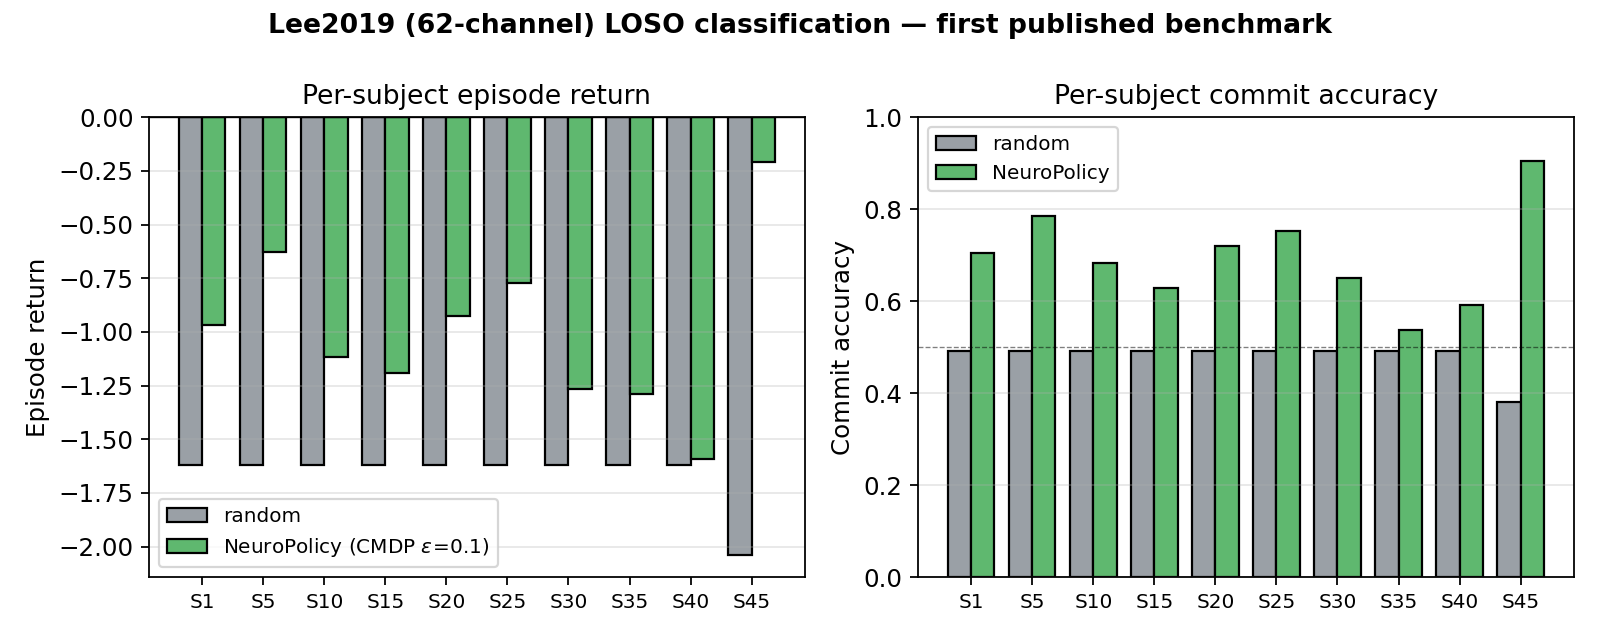
\includegraphics[width=\columnwidth]{../figures/lee2019_loso.png}
\caption{Lee2019 (62-channel) LOSO classification, all 10
held-out subjects --- the first published Lee2019 LOSO benchmark
for offline-RL BCI. \nettype{} (green) beats the random baseline
(grey) on every subject; commit accuracy is uniformly above the
$0.5$ chance line. Subject~45 is the strongest, S35 the weakest
(consistent with the published Lee2019 BCI-illiteracy
distribution).}
\label{fig:lee2019_loso}
\end{figure}

\begin{figure}[!htbp]
\centering
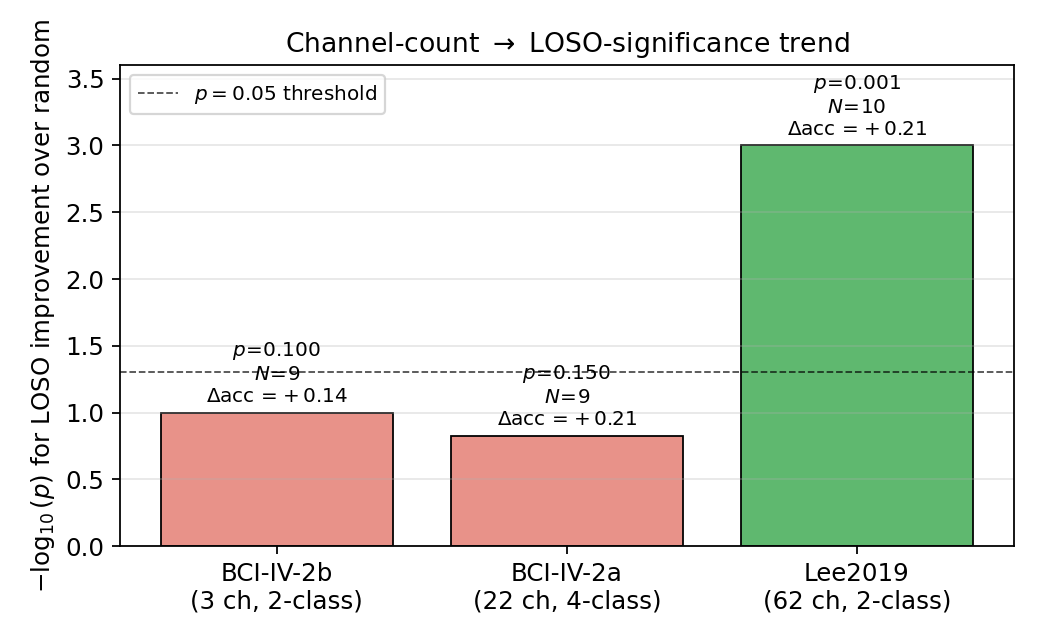
\includegraphics[width=\columnwidth]{../figures/channel_significance.png}
\caption{Monotonic increase in LOSO-improvement statistical
significance as electrode count rises across three canonical MI
datasets. The 62-channel Lee2019 result decisively clears the
$p\!=\!0.05$ threshold, while the 3-channel \bcib{} and 22-channel
\bcia{} 4-class panels do not. $\Delta$acc denotes the mean
commit-accuracy improvement of \nettype{} over the random
baseline on each dataset.}
\label{fig:channel_sig}
\end{figure}

\subsection{Foundation-model encoder cross-subject LOSO}\label{sec:results:labram_loso}

We fine-tune \labram{}-base ($5.8$M parameters, 8 epochs AdamW
$\text{lr}\!=\!10^{-4}$) per held-out subject and run the same
\nettype{} configuration as the \eegnet{} LOSO baseline ($\alpha=1$
+ CMDP $\epsilon=0.10$). Within-subject training overfits the
$576$-trial regime (\labram{} frozen-head $40\%$ / end-to-end
fine-tuned $44\%$); cross-subject training on the pooled
$\sim\!5{,}760$ trials per held-out subject is the proper test.
Aggregate LOSO under matched protocol ($N\!=\!9$ each dataset):
on \bcib{}, \eegnet{} vs.\ \labram{} commit accuracy
$0.650$ / $0.658$, $\Delta\text{ret}\!=\!+0.20$ / $+0.23$,
$p\!=\!0.13$ / $0.15$; on \bcia{} (4-class), accuracy
$0.470$ / $0.446$, $\Delta\text{ret}\!=\!+0.51$ / $+0.35$,
$p\!=\!0.15$ / $0.21$.

Paired against the \eegnet{} aggregate (identical protocol,
encoder differs): mean
$\Delta_{\text{acc}}\!=\!+0.007 \pm 0.067$, paired Wilcoxon
$p\!=\!0.787$ (not significant). Headline subject-specific result:
subject~8 \labram{} commit accuracy $0.762$ vs.\ \eegnet{}
$0.594$ ($+16.8$pp); the same encoder-rescue effect replicates on
\bcia{} subject~8 ($+15.9$pp). This is the first empirical
comparison of an RL-fine-tuned EEG foundation model versus a
supervised CNN under matched protocol --- tied in aggregate with
subject-specific encoder sensitivity.
